\documentclass[10pt,a4paper]{article}
\usepackage[utf8]{inputenc}
\usepackage[english]{babel}
\usepackage{amsmath}
\usepackage{amsfonts}
\usepackage{amssymb}
\usepackage{graphicx}
\usepackage{indentfirst}
\usepackage{fancyvrb}
\usepackage[hidelinks]{hyperref}
\author{Giuseppe L'Erario}
\date{}
\title{Principal Component Analysis}
\begin{document}
	\maketitle
	
	\section*{Introduction}
	The \emph{Principal Component Analysis} (PCA) is an unsupervised linear transformation technique used to reduce dimensionality of the data. 
	
	In this report the aim is to preprocess a set of images with PCA and then to train and test a \emph{Na\"ive Bayes Classifier}.
	
	\section{PCA}
	With PCA one can find the direction of maximum variance in high-dimensional data and then project these data onto a subspace with less dimension of the original data. 
	
	The principal components are the directions of the maximum variance, and they \emph{must} be orthogonal to each other (in other words, they must be uncorrelated). 
	
	The principal components are very sensitive to the scale of the data. It is useful indeed to \emph{normalize} the data (rescaling the features to a range of [0,1]) in order to analyze features of different scale, and \emph{standardize} them (center the mean to zero and the standard deviation to 1). 

	The pixels of every image are converted to matrix of values. This matrix is then reshaped into a vector.
	
	The commands used to read and preprocess data are:
	\begin{Verbatim}[obeytabs,tabsize=4]
		#creation of images file list
		for num in n_img:
			img_list += glob.glob(img_folder+str(num)+'_*')
		#conversion of the images
		for filename in img_list:
			im = np.asarray(Image.open(filename).convert("RGB"))
			im_raveled = np.ravel(im)
			img_data_raveled.append(im_raveled)
		#...and reshaping in 149152-dim vector
		X = np.array(img_data_raveled).reshape((len(img_list)), -1)
		#normalize and scaling
		X_std = preprocessing.scale(X)
	\end{Verbatim}  
	PCA algorithm:
	\begin{itemize}
		\item builds the covariance matrix;
		\item decomposes the covariance matrix in its eigenvectors and eigenvalues;
		\item return a matrix wich has as columns the eigenvectors associated to a eigenvalues (ordered from bigger to smaller). 
	\end{itemize}
	The bigger is the eigenvalue, the more is the variance associated to a feature.
	
	The aim is to train a classifier using less features, without loosing too much information. The results are:
	\begin{itemize}
		\item[-] less computation resources usage
		\item[-] less importance to "lightweight" features
	\end{itemize}
	PCA algorithm is performed easily with the \emph{sklearn} library:
	\begin{Verbatim}[obeytabs, tabsize=4]
		pca = PCA(value)
		X_PCA = pca.fit_transform(X_std)
	\end{Verbatim}	
	where \emph{value} is the number of the principal components.
	
	\subsection*{Plots}
	
	The results are shown by the plots. There are also the decision boundaries found by the classifier (explained later).
	
	\begin{figure}[ph]
	\centering
	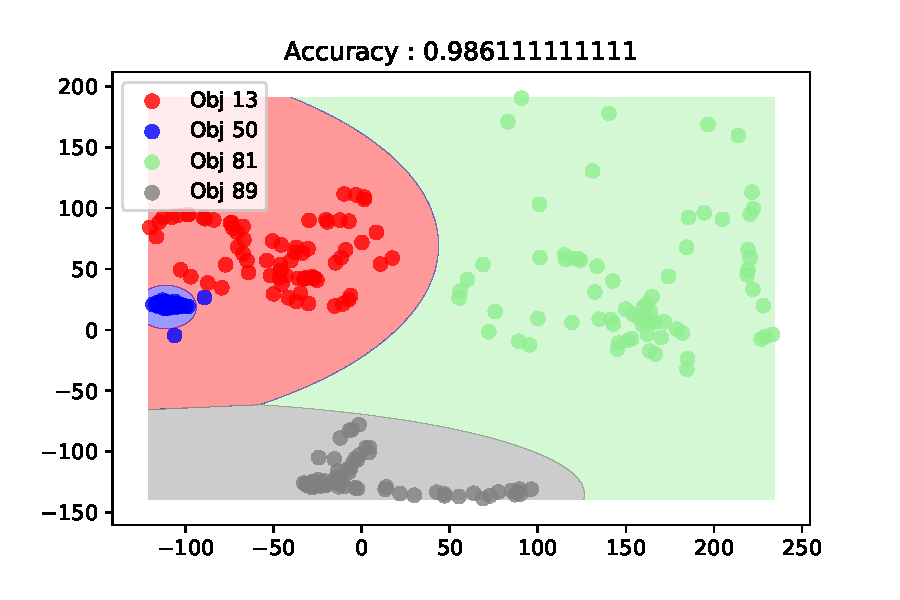
\includegraphics[width=0.7\linewidth]{../HW1/PCA2}
	\caption{First ancd second Principal Components}
	\label{fig:PCA2}
	\end{figure}

	\begin{figure}[ph]
	\centering
	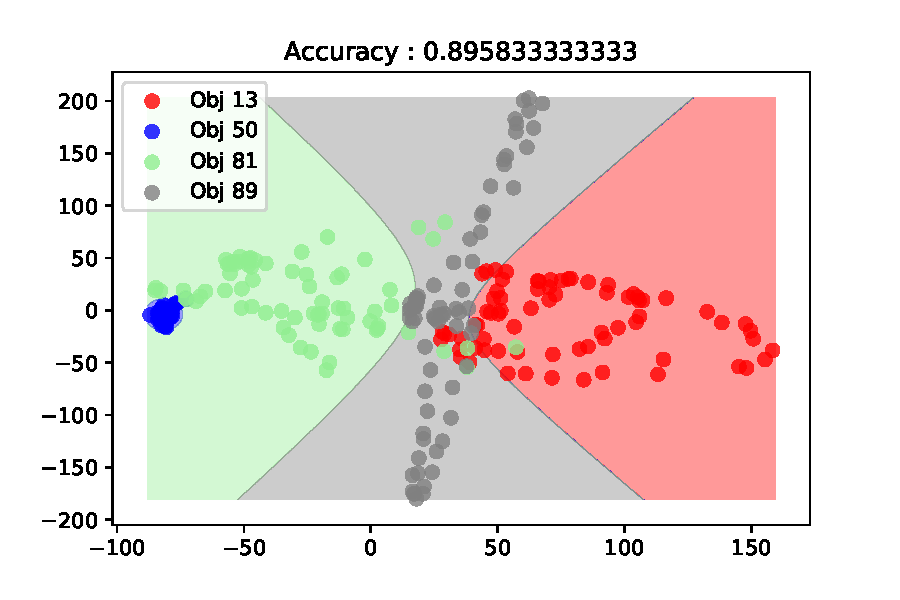
\includegraphics[width=0.7\linewidth]{../HW1/PCA4}
	\caption{Third and fourth PCs}
	\label{fig:PCA4}
	\end{figure}
	
	\begin{figure}[ph]
	\centering
	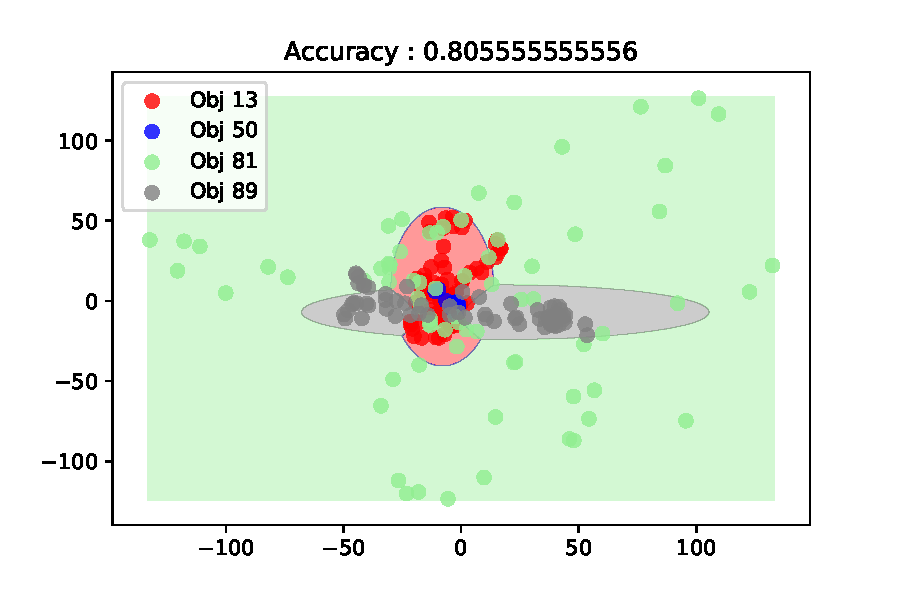
\includegraphics[width=0.7\linewidth]{../HW1/PCA11}
	\caption{Tenth and eleventh PCs}
	\label{fig:PCA11}
	\end{figure}
	
	It is possible to see in fig.\ref{fig:PCA2}, as expected, a good separation: the first two principal components bring with them the biggest part of the information.
	
	In fig.\ref{fig:PCA4} and fig.\ref{fig:PCA11} the classes are not well separated. These components are not so important to characterize the objects. In other words these features are similar among objects.
	
	We can see the "quantity" of information of every component described by the variance, in fig.\ref{fig:components}. The first two components got about 50\% of the information (\emph{cumulative explaindes variance}).
	
	\begin{figure}[ph]
	\centering
	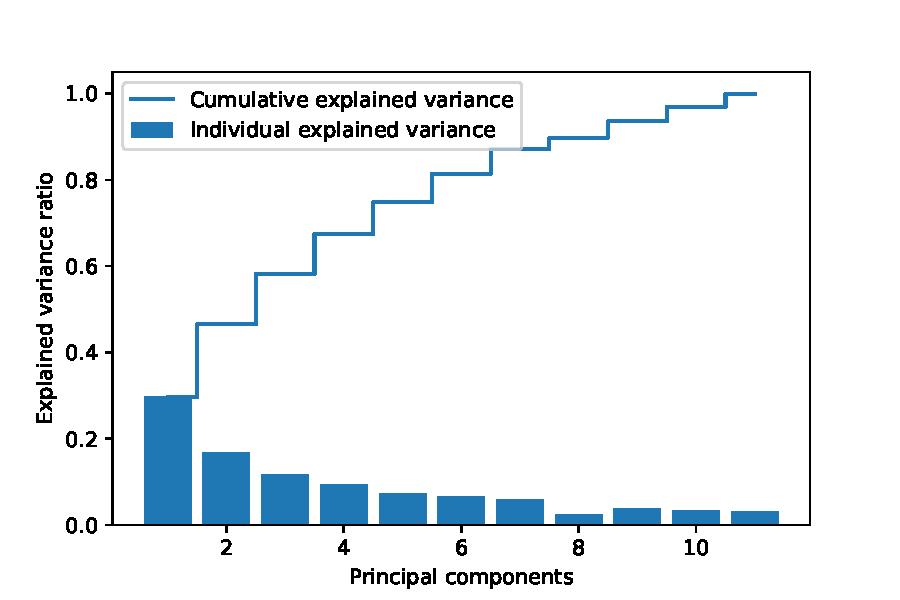
\includegraphics[width=0.7\linewidth]{../HW1/components}
	\caption{Variance of each Principal Component}
	\label{fig:components}
	\end{figure}

	\newpage
	
	\section{Na\"ive Bayes Classifier}
	
	The \emph{Na\"ive Bayes Classifier} are a class of probabilistic classifier based on Na\"ive Bayes rule.
	
	With this classifier is possible to determine the probability of an element to belong to a class of objects.
	
	We can use a classifier based on Gaussian distribution from \emph{sklearn} library:
	
	\begin{Verbatim}
	clf = GaussianNB()
	clf.fit(X_train, y_train)
	\end{Verbatim}
	
	where \emph{X\_train} and \emph{y\_train} are obtained through:
	
	\begin{Verbatim}
	X_train, X_test, y_train, y_test = 
		train_test_split(X_PCA, y, test_size=0.5)
	\end{Verbatim}
	
	With this command the dataset is divided in 2 separate datasets, one used to train the classifier and the second one used to test the accuracy of the trained classifier.	
	
	It can be seen in fig.\ref{fig:PCA2} that by using the first two principal components the classifier can achieve more than 90\% of accuracy. This result underlines what said before: the first two principal components have enough information to classify an object. 
	
	On the other side, using 3rd-4th and 10th-11th principal components the accuracy is considerably decreased: these features are useless for classification tasks.
 	
\end{document}